\documentclass[compress]{beamer}
\usepackage[brazil]{babel}
\usepackage[latin1]{inputenc}
\usepackage{amsmath}
\usepackage{graphicx}
\usepackage{listings}


%%%%%%%%%%%%%%%%%%%%%%%%%%%%%
% C O N F I G U R A � � E S %
%%%%%%%%%%%%%%%%%%%%%%%%%%%%%
\pdfpageattr {/Group << /S /Transparency /I true /CS /DeviceRGB>>}

\definecolor{listinggray}{gray}{0.9}
\definecolor{lbcolor}{rgb}{1,1,1}

\lstset{
	backgroundcolor=\color{lbcolor},
	tabsize=4,
	rulecolor=,
	language=matlab,
    basicstyle=\tiny,
    upquote=true,
    aboveskip={1.5\baselineskip},
    columns=fixed,
    showstringspaces=false,
    extendedchars=true,
    breaklines=true,
    prebreak = \raisebox{0ex}[0ex][0ex]{\ensuremath{\hookleftarrow}},
    frame=single,
    showtabs=false,
    showspaces=false,
    showstringspaces=false,
    identifierstyle=\ttfamily,
}

\renewcommand{\lstlistingname}{C�digo}
\renewcommand{\lstlistlistingname}{Lista de C�digos}

\usetheme{Ilmenau}
%vinho
%\usecolortheme[RGB={75,11,31}]{structure}
%verde
%\usecolortheme[RGB={35,75,11}]{structure}
%azul
\usecolortheme[RGB={149,188,44}]{structure}
\setbeamercovered{transparent}
\setbeamertemplate{blocks}[rounded][shadow=true]
\setlength{\tabcolsep}{1mm}
%\setbeamertemplate{footline}[frame number]
\setbeamertemplate{navigation symbols}{}
\setbeamertemplate{headline}[default]
\setbeamertemplate{footline}[default]
\setbeamertemplate{footline}{\hspace*{.5cm}\scriptsize{\hfill\vspace*{0.3cm}\insertframenumber\hspace*{.5cm}}}

\newenvironment{changemargin}[2]{%
  \begin{list}{}{%
    \setlength{\topsep}{0pt}%
    \setlength{\leftmargin}{#1}%
    \setlength{\rightmargin}{#2}%
    \setlength{\listparindent}{\parindent}%
    \setlength{\itemindent}{\parindent}%
    \setlength{\parsep}{\parskip}%
  }%
  \item[]}{\end{list}}

%%%%%%%%%%%
% C A P A %
%%%%%%%%%%%

%\title{T�cnicas de Planejamento para Gera��o de Planos de Execu��o em um Sistema Gerenciador de Fluxos de Trabalho Cient�fico}

\title{SERVLETS E JSP (JEE) - XHTML - Parte 2}

\author{Diogo Cezar Teixeira Batista \\
       {\footnotesize\ttfamily diogo@diogocezar.com.br} \\
       {\footnotesize\ttfamily http://www.diogocezar.com}
}

\institute{\large Universidade Tecnol�gica Federal do Paran� - UTFPR}

\date{Corn�lio Proc�pio - 2012}

\begin{document}

% %%%%%%%%%%%%%%%%%%%%%%%%%%%%%%
% S L I D E S  I N I C I A I S %
%%%%%%%%%%%%%%%%%%%%%%%%%%%%%%%%

\begin{frame}
    \titlepage
\end{frame}


%%%%%%%%%%%%%%%%%%%
% C O N T E � D O %
%%%%%%%%%%%%%%%%%%%

\section[XHTML - Parte 3]{XHTML - Parte 3}


\begin{frame}[c,allowframebreaks]
    \frametitle{XHTML - Manipulando Tabelas}
    \begin{itemize}
      \item os elementos \texttt{<table>} e \texttt{</table>} s�o respons�veis
pela manuten��o das tabelas nesta linguagem;
      \item uma c�lula pode se estender por mais de uma coluna, para isto deve
ser utilizado o atributo ``colspan'' seguido do n�mero de colunas que a c�lula
deve se expandir;
      \item caso a c�lula tenha de ocupar mais de uma linha o atributo a ser
utilizado � o ``rowspan'', ambos os atributos devem ser inseridos dentro de uma
declara��o \texttt{<td>} e \texttt{</td>}.
      \item na constru��o de uma tabela podemos utilizar alguns elementos;
      \item uma tabela ainda possui alguns atributos importantes;
    \end{itemize}
\end{frame}

\begin{frame}
    \frametitle{XHTML - Tabela Elementos}
    \begin{figure}[htb]
        \begin{center}
            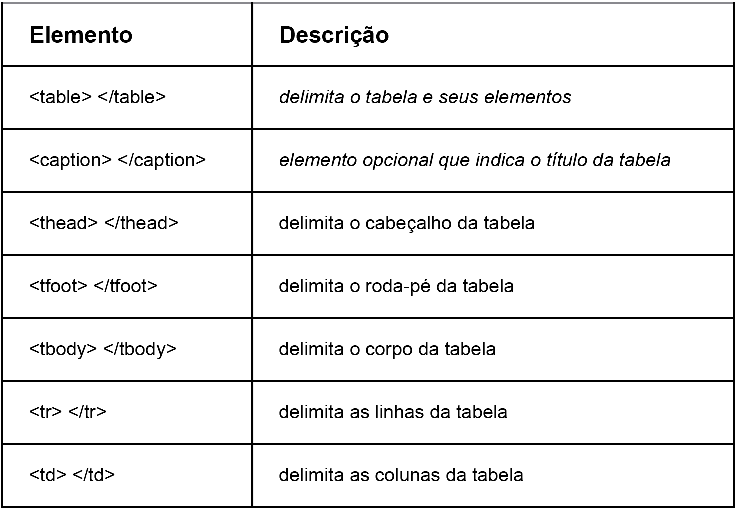
\includegraphics[width=10cm]{images/tabela-elementos.pdf}
        \end{center}
    \end{figure}
\end{frame}

\begin{frame}
    \frametitle{XHTML - Tabela Atributos}
    \begin{figure}[htb]
        \begin{center}
            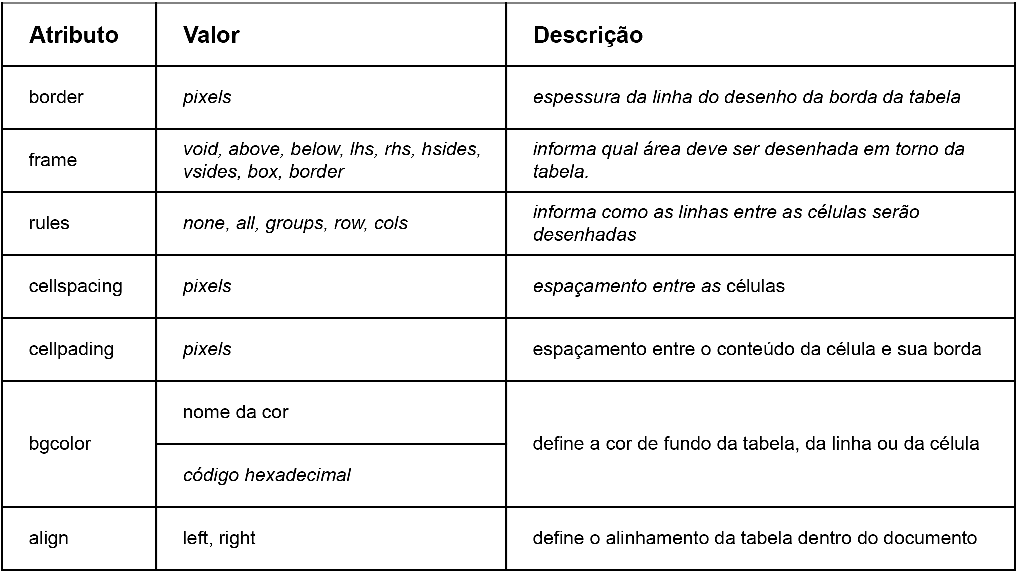
\includegraphics[width=10cm]{images/tabela-atributos.pdf}
        \end{center}
    \end{figure}
\end{frame}

\begin{frame}
    \frametitle{XHTML - Tabela - Exemplo}
    \lstinputlisting[language=HTML,label=tabela-1,
caption={Exemplo de Tabela}]{codes/XHTML_Tabela_1.txt}
\end{frame}

\begin{frame}
    \frametitle{XHTML - Tabela - Exemplo Uni�o C�lulas}
    \lstinputlisting[language=HTML,label=tabela-1,
caption={Exemplo de Tabela - Uni�o de C�lulas}]{codes/XHTML_Tabela_2.txt}
\end{frame}

\begin{frame}[c,allowframebreaks]
    \frametitle{XHTML - Imagens}
    \begin{itemize}
      \item atualmente os navegadores aceitam tr�s formatos de figuras: GIF,
JPEG e PNG;
      \item utiliza-se o elemento \texttt{<img>};
      \item atributo ``alt'' utilizado para fornecer um texto alternativo
quando a imagem n�o puder ser visualizada;
      \item atributo ``src'' utilizado para indicar a localiza��o da
figura;
      \item imagens png e gif podem ter o fundo transparente;
      \item as imagens refer�ntes ao layout de uma p�gina n�o s�o manipuladas
pela tag \texttt{<img>}, s�o adicionadas no arquivos CSS;
      \item As imagens possuem alguns atributos importatens;
    \end{itemize}
\end{frame}

\begin{frame}
    \frametitle{XHTML - Imagens Atributos}
    \begin{figure}[htb]
        \begin{center}
            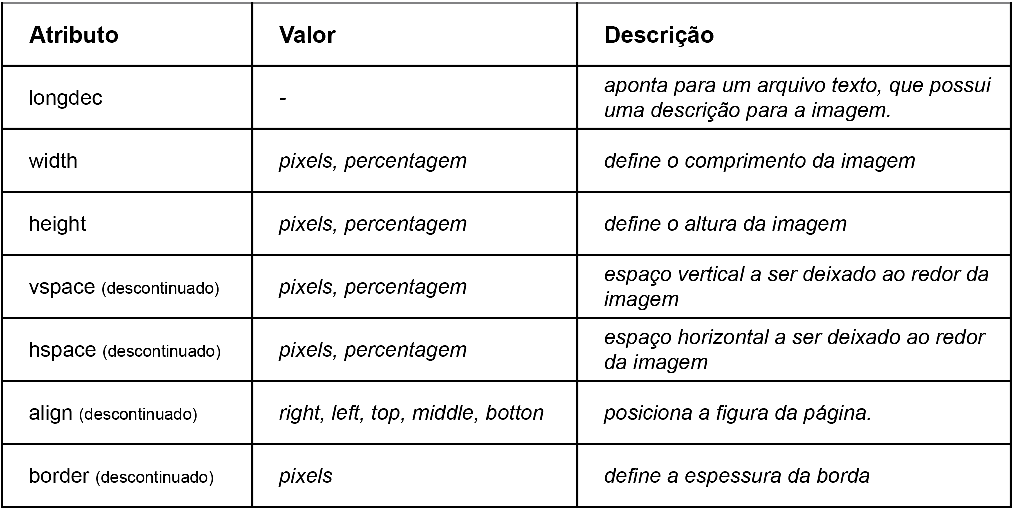
\includegraphics[width=10cm]{images/imagem-atributos.pdf}
        \end{center}
    \end{figure}
\end{frame}

\begin{frame}
    \frametitle{XHTML - Imagem - Exemplo}
    \lstinputlisting[language=HTML,label=tabela-1,
caption={Exemplo de Imagem}]{codes/XHTML_Imagem.txt}
\end{frame}

\begin{frame}[c,allowframebreaks]
    \frametitle{XHTML - Formul�rios}
    \begin{itemize}
      \item os formul�rios s�o utilizados para o envio de informa��es ao
servidor ou para a intera��o da p�gina com o usu�rio atrav�s do uso de
JavaScripts;
      \item os dados podem ser submetidos atrav�s de dois m�todos \textbf{GET} e
\textbf{POST}:
      \begin{itemize}
       \item \textit{GET}: os dados ser�o anexados � URL e enviados ao servidor;
       \item \textit{POST}: envia os dados junto com as demais informa��es
contidas no cabe�alho do HTTP;
      \end{itemize}
      \framebreak
      \item ao contr�rio do \textit{POST} que pode manipula qualquer quantidade
de informa��es, o \textit{GET} fica limitado pelo tamanho m�ximo permitido para
uma URL;
      \item O \textit{GET} � menos seguro, mas seu uso permite o reenvio de um
formul�rio sem que o mesmo seja re-digitado;
      \item O \textit{GET} pode funcionar como um controle para exibi��o do
conte�do de uma mesma p�gina;
      \item para a constru��o dos formul�rios devemos fazer uso dos elementos
\texttt{<form>} e \texttt{</form>}, que possuem os seguintes atributos:
    \end{itemize}
\end{frame}

\begin{frame}
    \frametitle{XHTML - Formul�rio Atributos}
    \begin{figure}[htb]
        \begin{center}
            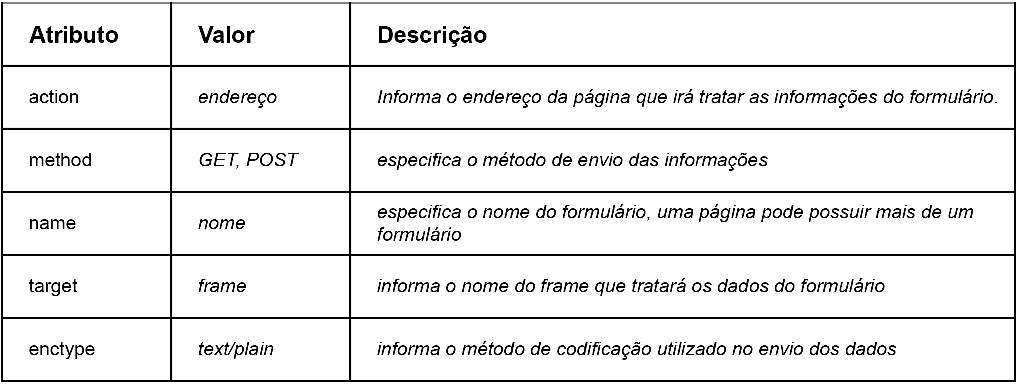
\includegraphics[width=10cm]{images/form-atributos.pdf}
        \end{center}
    \end{figure}
\end{frame}

\begin{frame}
    \frametitle{XHTML - Formul�rio Input}
    \begin{itemize}
     \item Para armazenar as informa��es fornecidas pelo usu�rio podemos fazer
uso do elemento \texttt{<input />} , que possui os seguintes atributos:
    \end{itemize}
    \begin{figure}[htb]
        \begin{center}
            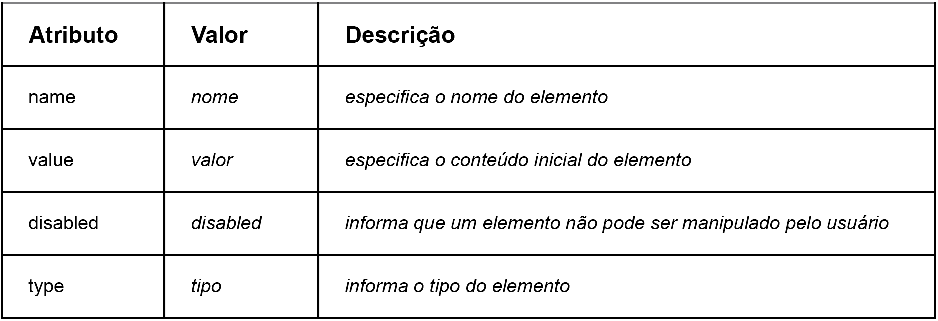
\includegraphics[width=10cm]{images/input-atributos.pdf}
        \end{center}
    \end{figure}
\end{frame}

\begin{frame}[c,allowframebreaks]
    \frametitle{XHTML - Formul�rio Input}
    \begin{itemize}
     \item os principais tipos do elemento ``input'' s�o:
    \end{itemize}
    \begin{figure}[htb]
        \begin{center}
            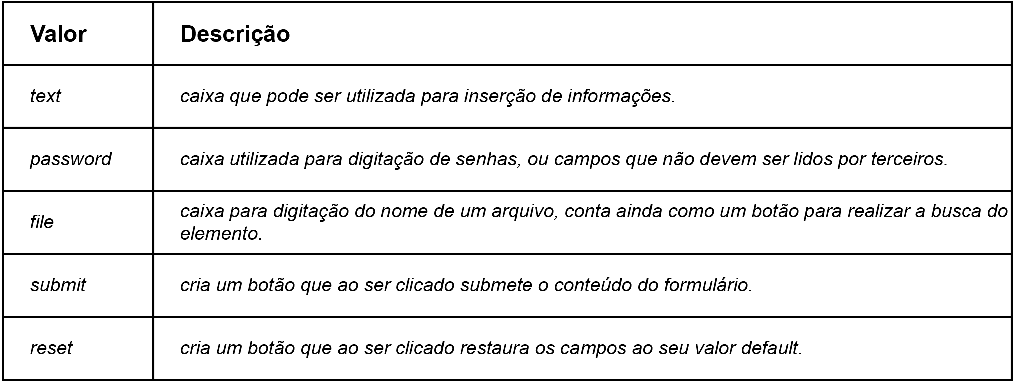
\includegraphics[width=10cm]{images/tipo-input-1.pdf}
        \end{center}
    \end{figure}
    \framebreak
    \begin{figure}[htb]
        \begin{center}
            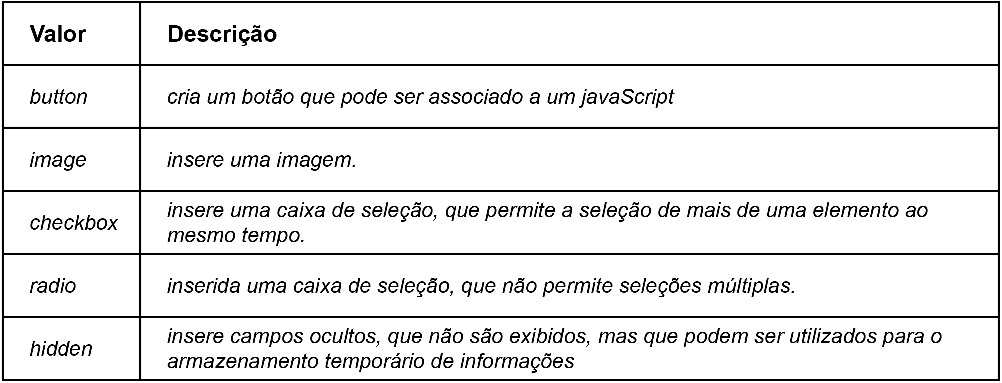
\includegraphics[width=10cm]{images/tipo-input-2.pdf}
        \end{center}
    \end{figure}
\end{frame}

\begin{frame}
    \frametitle{XHTML - Formul�rio Input - Text}
    \begin{itemize}
     \item o elemento ``input'' do tipo \textit{text}, possui os atributos:
    \end{itemize}
    \begin{figure}[htb]
        \begin{center}
            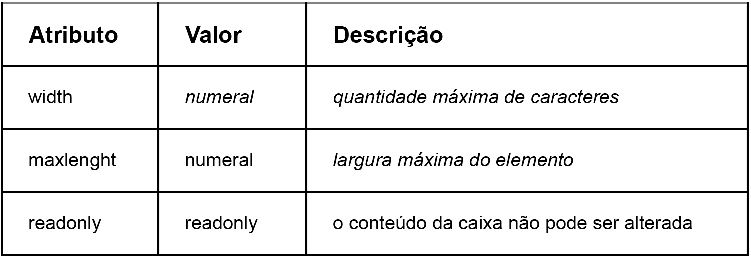
\includegraphics[width=10cm]{images/input-text.pdf}
        \end{center}
    \end{figure}
\end{frame}

\begin{frame}
    \frametitle{XHTML - Formul�rio Input - Buttom}
    \begin{itemize}
     \item o elemento ``input'' do tipo \textit{buttom}, possui os atributos:
    \end{itemize}
    \begin{figure}[htb]
        \begin{center}
            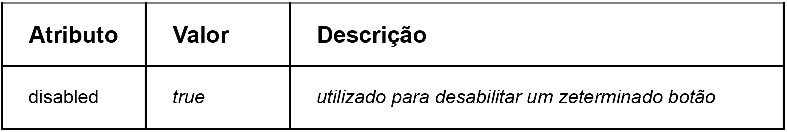
\includegraphics[width=10cm]{images/input-buttom.pdf}
        \end{center}
    \end{figure}
\end{frame}

\begin{frame}
    \frametitle{XHTML - Formul�rio Input - Select}
    \begin{itemize}
     \item o elemento ``input'' do tipo \textit{select}, possui os atributos:
    \end{itemize}
    \begin{figure}[htb]
        \begin{center}
            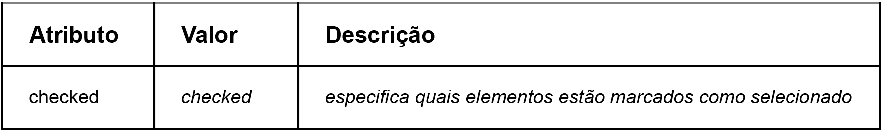
\includegraphics[width=10cm]{images/input-selecao.pdf}
        \end{center}
    \end{figure}
\end{frame}

\begin{frame}
    \frametitle{XHTML - Formul�rio Input - Lista de Sele��o}
    \begin{itemize}
     \item para a cria��o de uma lista para sele��o devemos utilizar
o elemento \texttt{<select>} \texttt{</select>};
    \item e o elemento \texttt{<option>} \texttt{</option>} � utilizado na
defini��o de cada item da lista.
    \end{itemize}
        \lstinputlisting[language=HTML,label=selecao-1,
caption={Exemplo de Lista de Sele��o}]{codes/XHTML_Selecao.txt}
\end{frame}

\begin{frame}
    \frametitle{XHTML - Formul�rio Input - Radio}
    \begin{itemize}
     \item utilizado para determinar a escolha de uma �nica op��o;
     \item para agrupar os radios utiliza-se o mesmo atributo ``name'';
     \item o atributo ``value'' indica o valor do grupo;
    \end{itemize}
        \lstinputlisting[language=HTML,label=radio-1,
caption={Exemplo de Radio}]{codes/XHTML_Radio.txt}
\end{frame}

\begin{frame}
    \frametitle{XHTML - Formul�rio Input - Checkbox}
    \begin{itemize}
     \item utilizado para marcar determinada op��o;
     \item para agrupar os checkbox utiliza-se o mesmo atributo ``name'';
     \item o atributo ``value'' indica o valor do grupo;
     \item pode-se marcar v�rios elementos de um mesmo grupo;
    \end{itemize}
        \lstinputlisting[language=HTML,label=heckbox-1,
caption={Exemplo de Checkbox}]{codes/XHTML_Checkbox.txt}
\end{frame}

\begin{frame}
    \frametitle{XHTML - Formul�rio Input - TextArea}
    \begin{itemize}
     \item outro elemento para inser��o informa��es � o \texttt{<textarea>}
\texttt{</textarea>}. Ele permite a inser��o de v�rias linhas, possui os
atributos:
    \end{itemize}
    \begin{figure}[htb]
        \begin{center}
            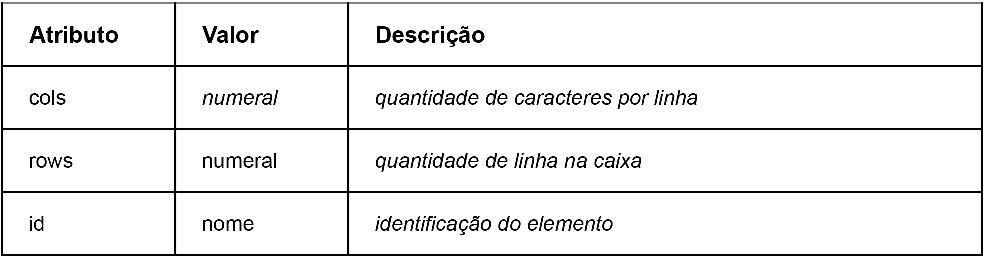
\includegraphics[width=10cm]{images/form-textarea.pdf}
        \end{center}
    \end{figure}
\end{frame}

\begin{frame}
    \frametitle{Atividades}
    \begin{itemize}
      \item fa�a uma p�gina em \texttt{XHTML} utilizando:
      \begin{itemize}
	\item uma tabela de dias da semana;
	\item uma tabela com duas c�lulas mescladas;
	\item uma imagem;
	\item um formul�rio com:
	\begin{itemize}
	 \item \textit{input} do tipo \textit{text};
	 \item \textit{input} do tipo \textit{password};
	 \item \textit{input} do tipo \textit{buttom};
	 \item op��es com \textit{radio buttom};
	 \item op��es com \textit{checkbox};
	 \item \textit{combobox} de op��es;
	 \item \textit{textarea};
	\end{itemize}
      \end{itemize}
    \end{itemize}
\end{frame}




\end{document}